\documentclass[12pt]{article}
\usepackage{graphicx}

\begin{document}

  \title{Note de vulnérabilité - Reverse challenge}
  \author{Kerchouche Fatiha - Haral Dylan - Francio François - Clément Lyonnet}
  \date{}
  \maketitle

  Lors de l'analyse d'exécutables, il a été possible de retrouver le mot de passe demandé par celui-ci.

  \section{Vulnérabilité(s)}
  \begin{itemize}
    \item Les codes exécutables contiennent des informations sur le mot de passe à entrer.
    \item Le flag ainsi retrouvé est "3004".
  \end{itemize}

  \section{Méthode(s)}
  \begin{itemize}
    \item En désassemblant le premier exécutable, il a été possible d'analyser le comportement de celui-ci.
    \item Il a été possible de voir que \texttt{exe1} fait appel à \texttt{exe2} (voir Annexes plus bas).
    \item En désassemblant \texttt{exe2}, les caractères du mot de passe demandé sont ainsi retrouvés.
    \item Une fois le mot de passe correct entré à \texttt{exe1}, celui-ci télécharge un autre exécutable qui génère le fichier contenant le flag.
  \end{itemize}

  \newpage

  \section{Annexes}
  L'appel à \texttt{exe2} depuis \texttt{exe1} : \\
  \\
  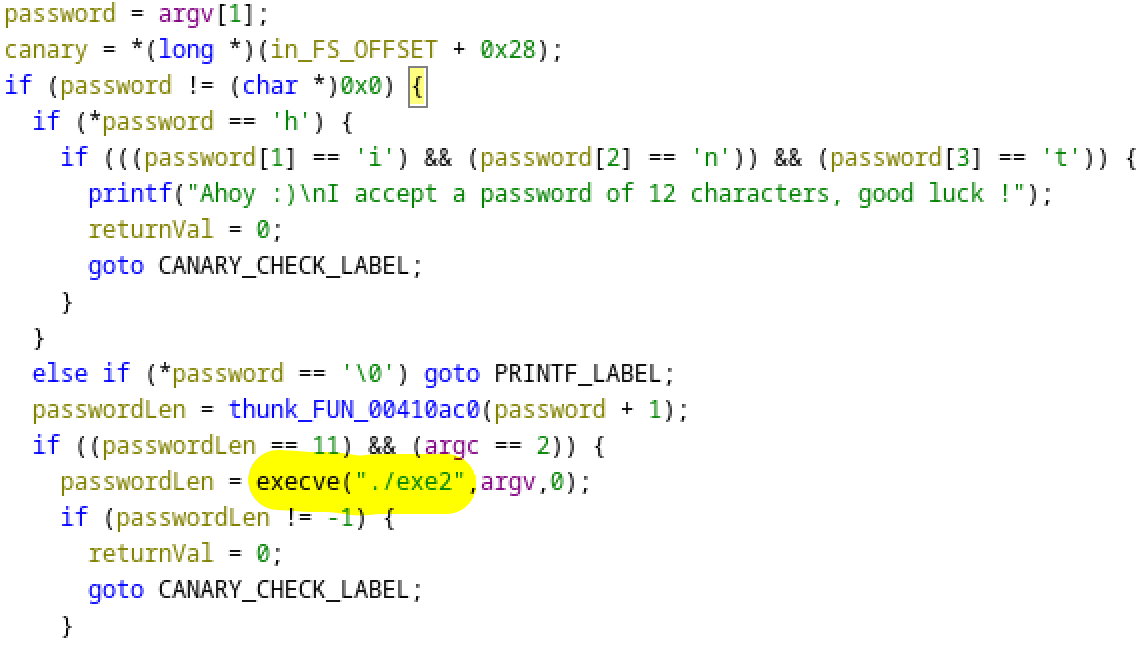
\includegraphics{"./1.png"}\\
  \\
  Les caractères du mot de passe retrouvés dans \texttt{exe2} : \\
  \\
  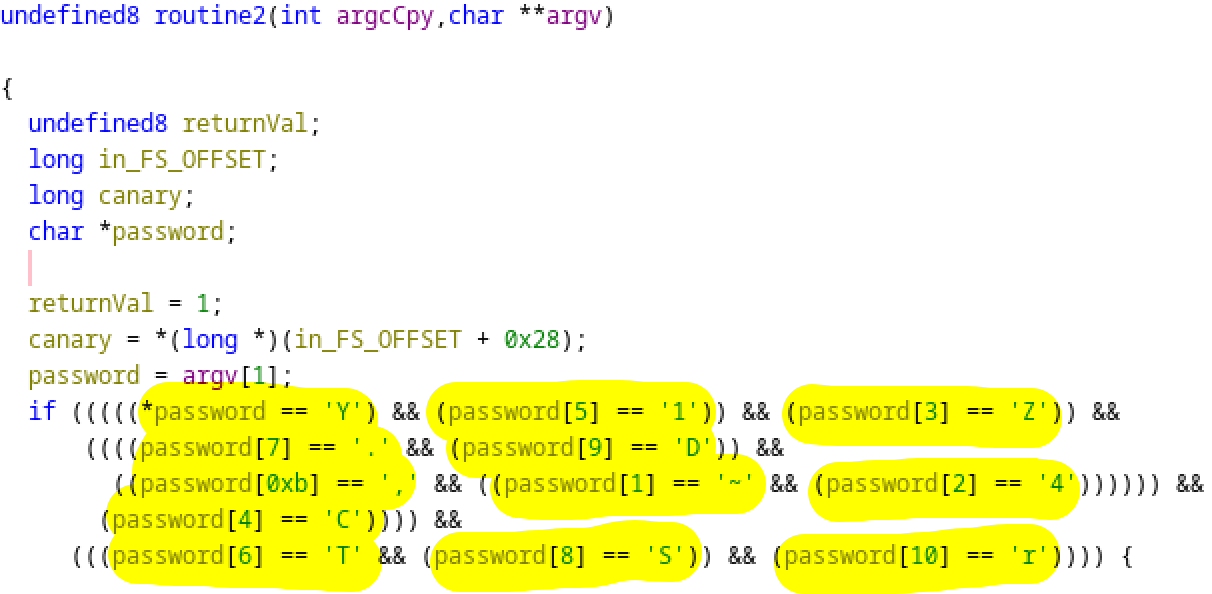
\includegraphics{"./2.png"}
 
  \newpage

  L'analyse de \texttt{exe2} révèle l'exécution de \texttt{exe3} : \\
  \\
  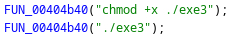
\includegraphics{"./3.png"}\\
  \\
  Le flag est retrouvé sous forme de GIF : \\
  \\
  
\includegraphics{"./4.png"}

\end{document}
